\documentclass[a4paper]{article}

\usepackage[T1]{fontenc}	
\usepackage{amsmath}
\usepackage{amssymb}
\usepackage{fancyhdr}
\usepackage{booktabs}
\usepackage{graphicx}

\pagestyle{fancy}
\rhead{Home Assignment 1}
\lhead{Noah Hansson \& Kristoffer Nordström}

\begin{document}
 
\section*{Random Number Generation}

\subsection*{a)}
We are intrested in finding the conditional distribution function of a stochastic variable $X$ given that $X$ is within a given interval, i.e $F_{X|X\in I}(x)$, where I is the closed interval $I = [a,b]$. Using the law of total probability we can express this as
\begin{equation}
    F_{X|X\in{I}}(x) = \frac{\int_a^xf_X(x)dx}{c} = \frac{\int_a^xf_X(x)dx}{\int_a^bf_X(x)dx} = \frac{F_X(x)-F_X(a)}{F_X(b)-F_X(a)}
\end{equation}
From this we can easily compute the conditional probability density function
\begin{equation}
    f_{X|X\in{I}}(x) = \frac{dF_{X|X\in{I}}(x)}{dx} = \frac{f_X(x)}{F_X(b)-F_X(a)}
\end{equation}

\subsection*{b)}
By the definition of an inverse distribution we want to find a probability distribution function $F_{X|X \in I}^{-1}(u)$ such as:
\begin{equation}
    F_{X|X \in I}(F_{X|X \in I}^{-1}(u)) = u
\end{equation}
where $u$ is a variable sampled from a uniform distribution $u \sim U[0,1]$. Inserting our expression for $F_{X|X \in I}(x)$ gives us
\begin{equation}
    \frac{F_X(F_{X|X\in I}^{-1}(u))-F_X(a)}{F_X(b)-F_X(a)} = u
\end{equation}
Solving for $F_{X|X\in I}^{-1}(x)$ gives us
\begin{equation}
    F_{X|X\in I}^{-1}(u) = F_X^{-1}((F_X(b)-F_X(a))u + F_X(a))
\end{equation}


\newpage
\section*{Power Production of a Wind Turbine}

\subsection*{a) Crude Monte-Carlo sampling}
To calculate an initial estimate of the power production of the Wind Turbine we start by sampling the power production using regular Monte-Carlo sampling. We begin by generating $10^5$ samples of wind distributed by a Weibull distribution. We then calculate the generated power for each wind sample and then find the average and the variance for each month. The estimate is calculated as follows:
\begin{equation}
    \tau = \mathbb{E}[\phi(X)] = \frac{1}{N}\sum_{i = 1}^N\phi(X_i)
\end{equation}
And since the sample size is large we can also assume that the central limit theorem applies, giving us:
\begin{equation}
    \mathbb{V}[\sqrt{N}(\tau_N-\tau)] = N\mathbb{V}[\tau_N-\tau] = \mathbb{V}[\phi(X)]
\end{equation}
In this case the stochastic variable $X$ is the wind speed and $\phi(X)$ is the power curve function for the wind turbine.

The results are presented in table \ref{tab:CrudeResults} and the samples for january are plotted in figure \ref{fig:samplesJan}.
\begin{table}
    \centering
    \caption{Crude Monte Carlo estimates and confidence intervals of power production for each month of the year}
    \label{tab:CrudeResults}
    \begin{tabular}{lllr}
\toprule
{} &   Mean [kW] &        Interval &     Variance  \\
Month &             &                 &               \\
\midrule
jan   &  1729398.04 &   $\pm$ 7586.68 &  1.498275e+12 \\
feb   &  1574090.66 &   $\pm$ 7528.13 &  1.475237e+12 \\
mar   &  1466612.49 &   $\pm$ 7426.44 &  1.435653e+12 \\
apr   &  1190918.98 &   $\pm$ 7107.77 &  1.315086e+12 \\
may   &  1139016.09 &   $\pm$ 6969.14 &  1.264290e+12 \\
jun   &  1210539.74 &   $\pm$ 7135.69 &  1.325438e+12 \\
jul   &  1143510.67 &   $\pm$ 7000.18 &  1.275577e+12 \\
aug   &  1213284.01 &   $\pm$ 7149.09 &  1.330423e+12 \\
sep   &  1444936.39 &   $\pm$ 7415.53 &  1.431438e+12 \\
oct   &  1586902.48 &   $\pm$ 7629.18 &  1.515106e+12 \\
nov   &  1731424.95 &   $\pm$ 7584.78 &  1.497524e+12 \\
dec   &  1722549.05 &   $\pm$ 7586.04 &  1.498021e+12 \\
\bottomrule
\end{tabular}

\end{table}

\begin{figure}
    \centering
    \caption{Sampled wind speed (left) and power production (right) for January}
    \label{fig:samplesJan}
    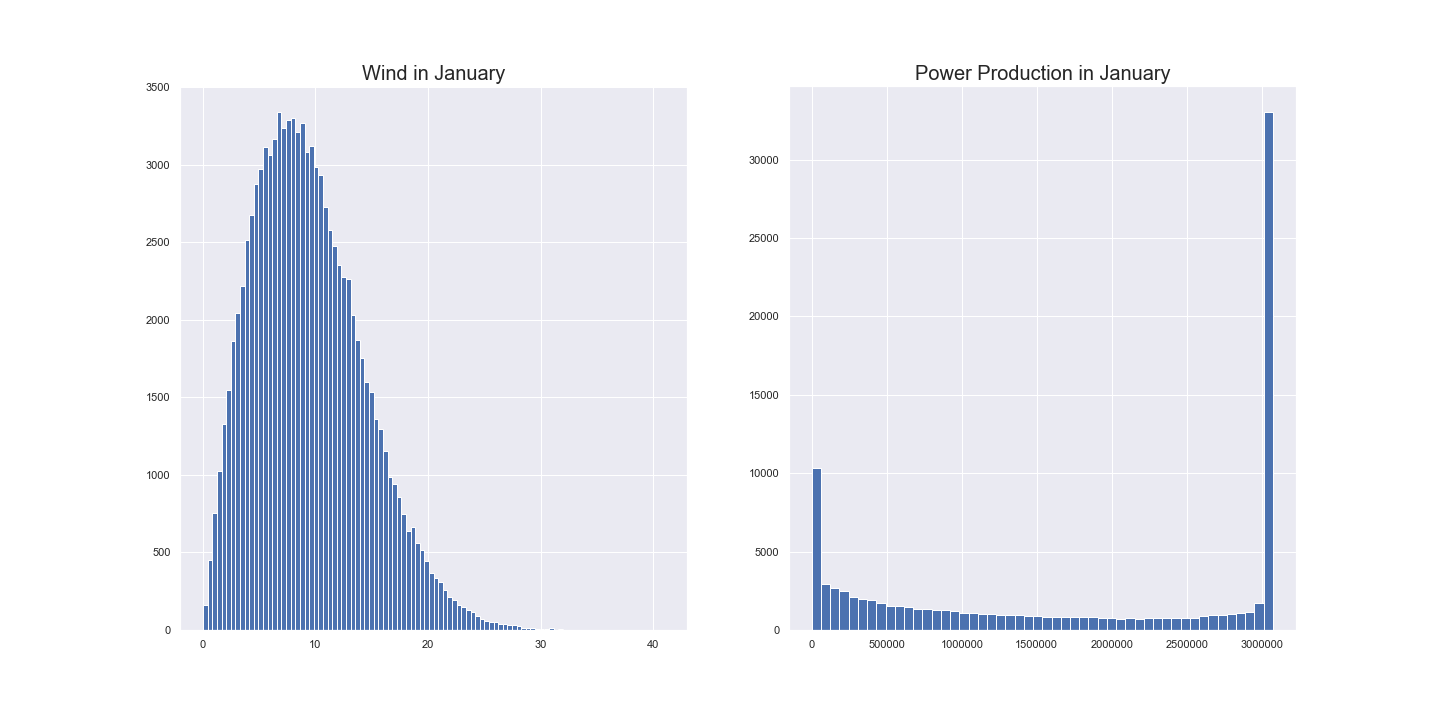
\includegraphics[width = 1.0\textwidth]{janCrude}
\end{figure}

\textbf{TRUNCATED VERSION}

\begin{table}
    \centering
    \caption{Crude truncated Monte Carlo estimates and confidence intervals of power production for each month of the year}
    \label{tab:CrudeTruncatedResults}
    \begin{tabular}{lllr}
\toprule
{} & $\tau$ [kW] &      $I_{95\%}$ &  $\mathbb{V}(\tau)$ \\
Month &             &                 &                     \\
\midrule
jan   &  1731719.18 &   $\pm$ 6597.59 &        1.133075e+12 \\
feb   &  1566574.66 &   $\pm$ 6533.15 &        1.111049e+12 \\
mar   &  1466464.51 &   $\pm$ 6426.78 &        1.075165e+12 \\
apr   &  1192070.88 &   $\pm$ 5940.35 &        9.185679e+11 \\
may   &  1135596.02 &   $\pm$ 5830.83 &        8.850116e+11 \\
jun   &  1211715.53 &    $\pm$ 5994.8 &        9.354866e+11 \\
jul   &  1147073.32 &   $\pm$ 5838.47 &        8.873321e+11 \\
aug   &  1211018.41 &   $\pm$ 5992.59 &        9.347962e+11 \\
sep   &  1446737.76 &   $\pm$ 6390.57 &        1.063082e+12 \\
oct   &  1585950.52 &    $\pm$ 6531.4 &        1.110452e+12 \\
nov   &  1731702.22 &   $\pm$ 6609.87 &        1.137295e+12 \\
dec   &  1726024.48 &   $\pm$ 6602.99 &        1.134929e+12 \\
\bottomrule
\end{tabular}

\end{table}

\begin{figure}
    \centering
    \caption{Sampled truncated wind speed (left) and power production (right) for January}
    \label{fig:samplesTruncJan}
    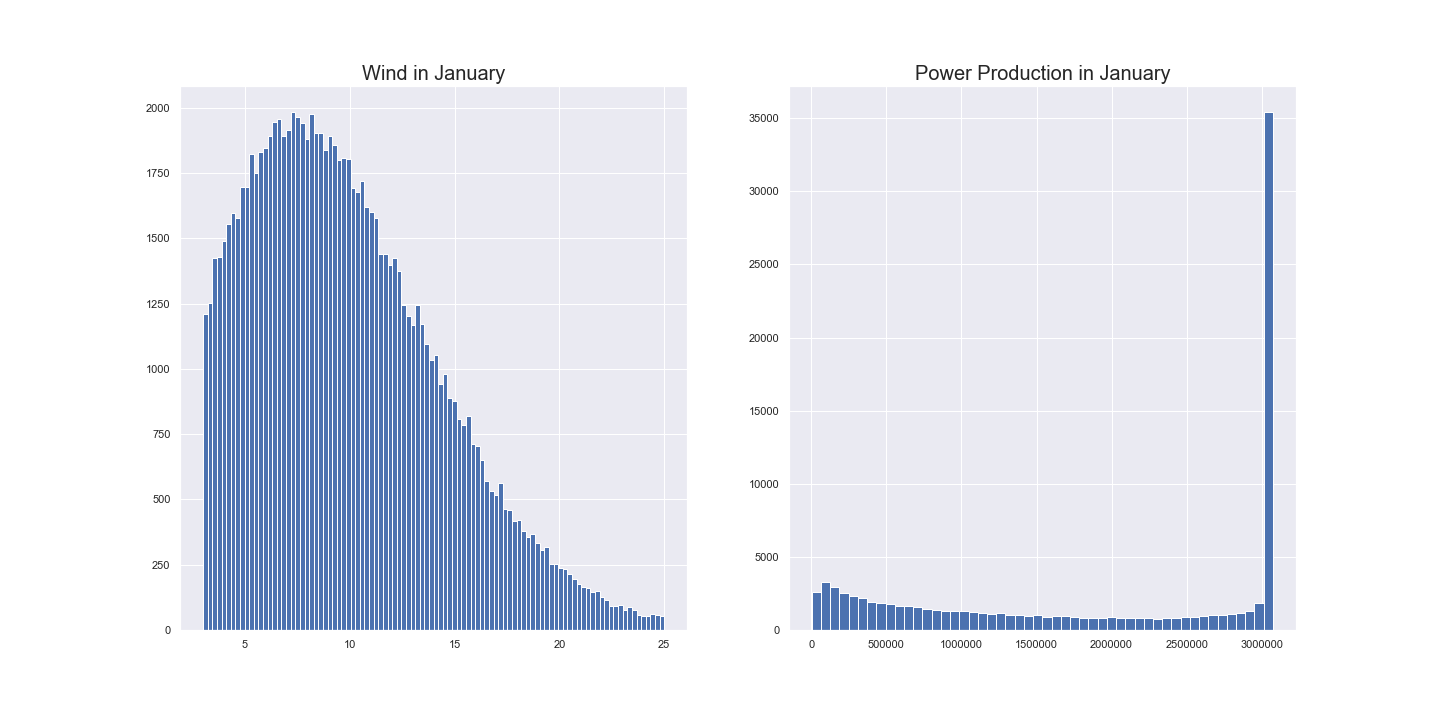
\includegraphics[width = 1.0\textwidth]{janCrudeTrunc}
\end{figure}

\subsection*{b) Importance Sampling}
To reduce the variance of the Monte-Carlo estimate we will here apply the importance sampling method. When we generate random wind samples we sometimes get samples of wind speed that give us a power production of zero. These samples give do not help finding a better estimate of the average power, as they only increase the variance of the estimator. Instead, we try to find an instrumental density g where we then draw our wind samples from. This reduces the amount of "bad" samples and reduces the variance of the estimator. \noindent To find an estimate of the average power production we use the following calculations, where the density $g(x)$ is a density such as $g(x) = 0 \rightarrow \phi(x)f(x) = 0$
\begin{equation}
    \begin{gathered}
        \tau = \mathbb{E}_f(\phi(X)) = \int_{|\phi(x)|f(x)>0}\phi(x)f(x)dx = \int_{g(x)>0}\phi(x)\frac{f(x)}{g(x)}g(x)dx = \\
        = \mathbb{E}_g[\phi(x)\frac{f(x)}{g(x)}] = \mathbb{E}_g[\phi(X)\omega(X)]
    \end{gathered}
\end{equation}
where
\begin{equation}
    \omega : \{x \in X : g(x)>0 \} \ni x \rightarrow \frac{f(x)}{g(x)}
\end{equation}
This gives us the estimates of $\tau$ as
\begin{equation}
    \tau = \mathbb{E}_g[\phi(X)\omega(X)]
\end{equation}
with the variance
\begin{equation}
    \mathbb{V}[\tau_N] = \frac{1}{N}\mathbb{V}_g[\phi(X)\omega(X)]
\end{equation}

In practice, we aim at finding a distribution $g(x)$ that resembles $f(x)\phi(x)$ and has a support that includes the whole support of $f(x)\phi(x)$. We then fine tune $g(x)$ such that the function $\phi(x)\omega(x)$ is close to constant in the support of $g(x)$. We then draw $10^5$ samples from $g(x)$ as the stochastic variable $X$ to estimate $\tau$. The results are presented in table \ref{tab:ISresults}.

\begin{table}
    \centering
    \caption{Importance Sampling Monte Carlo estimates and confidence intervals of power production for each month of the year}
    \label{tab:ISresults}
    \begin{tabular}{lll}
\toprule
Month & $\tau$ [kW] &   $I_{95\%}$ \\
\midrule
  Jan &     1730.18 &   $\pm$ 3.02 \\
  Feb &     1570.83 &   $\pm$ 2.68 \\
  Mar &     1468.02 &   $\pm$ 2.56 \\
  Apr &     1187.48 &    $\pm$ 2.5 \\
  May &     1138.65 &   $\pm$ 2.43 \\
  Jun &     1211.77 &   $\pm$ 2.54 \\
  Jul &     1141.39 &   $\pm$ 2.42 \\
  Aug &     1211.93 &   $\pm$ 2.53 \\
  Sep &     1447.62 &   $\pm$ 2.55 \\
  Oct &     1587.56 &   $\pm$ 2.75 \\
  Nov &     1730.17 &   $\pm$ 3.04 \\
  Dec &     1731.64 &   $\pm$ 3.02 \\
\bottomrule
\end{tabular}

\end{table}

\begin{figure}
    \centering
    \caption{$g(x)$ (scale-transformed) and $\phi(x)*f_X(x)$ (left) and $\omega(x)$ (right) for January}
    \label{fig:ISMCjan}
    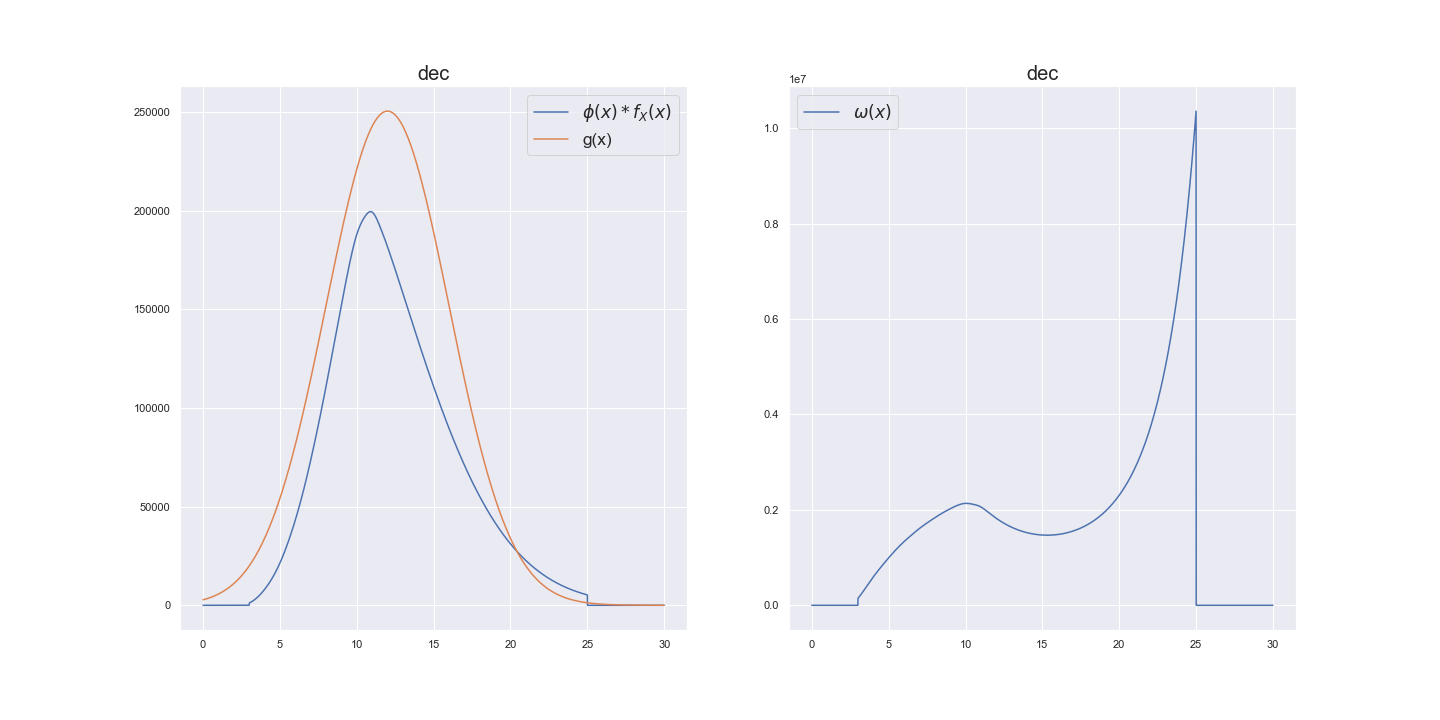
\includegraphics[width = 1.0\textwidth]{janISMC}
\end{figure}

\subsection*{c) Antithetic sampling}
Another method of reducing the variance is to use antithetic sampling to estimate $\tau = \mathbb{E}_f[\phi (X)]$ by defining the variable $V \overset{\mathrm{def}}{=} \phi (X)$ so that $\tau = \mathbb{E}[V]$. Then we find another variable $V^\prime$ with the same mean and distribution as $V$, but with a negative covariance. Then, if we define $$W \overset{\mathrm{def}}{=} \frac{V + V^\prime}{2}$$ it holds that $\mathbb{E}[W] = \tau$ and $$\mathbb{V}[W] = \frac{1}{2}(\mathbb{V}[V] + \mathbb{C}[V, V^\prime])$$Since the covariance between $V$ and $V^\prime$ is negative we should be able to find an estimate of $\tau$ with a lower variance than when using crude Monte Carlo.

In this case, we find $V$ and $V^\prime$ by evaluating the power fuction $P(V)$ of sampled wind using the inverse conditional weibull distribution. This gives us
\begin{equation}
    V = P(F_{X|X\in I}^{-1}(u))
\end{equation}
and
\begin{equation}
    V^\prime = P(F_{X|X\in I}^{-1}(1-u))
\end{equation}

Generating $10^5$ samples of $u$ and running each sample through both inverse distributions before avaluating the power production from those samples gives us the two stochastic variables $V$ and $V^\prime$ This gives us two identically distributed wind samples with negative covariance. The results are presented in table \ref{tab:ATresults}.

\begin{table}
    \centering
    \caption{Antithetic Monte Carlo estimates and confidence intervals of power production for each month of the year}
    \label{tab:ATresults}
    \begin{tabular}{lllr}
\toprule
{} &        Mean &       Interval &      Variance \\
Month &             &                &               \\
\midrule
jan   &  1731209.36 &  $\pm$ 1216.66 &  3.853263e+10 \\
feb   &  1570160.14 &   $\pm$ 528.83 &  7.279768e+09 \\
mar   &  1468632.69 &   $\pm$ 451.58 &  5.308426e+09 \\
apr   &   1189182.4 &  $\pm$ 1133.65 &  3.345366e+10 \\
may   &   1139511.5 &  $\pm$ 1250.12 &  4.068096e+10 \\
jun   &  1213083.74 &  $\pm$ 1071.68 &  2.989610e+10 \\
jul   &  1140040.78 &  $\pm$ 1249.86 &  4.066400e+10 \\
aug   &  1213048.25 &  $\pm$ 1072.04 &  2.991646e+10 \\
sep   &  1446315.35 &   $\pm$ 487.86 &  6.195647e+09 \\
oct   &  1585782.69 &   $\pm$ 662.37 &  1.142059e+10 \\
nov   &   1730221.5 &  $\pm$ 1215.95 &  3.848735e+10 \\
dec   &  1731120.96 &  $\pm$ 1214.81 &  3.841545e+10 \\
\bottomrule
\end{tabular}

\end{table}

\subsection*{d) Probability of power production}
To find the probability of the wind turbine producing power, $\mathbb{P}(P(V) > 0)$, we can simply use the weibull probability distribution function. Since the turbine only produces power when the wind is between 3 and 25 m/s we can express this as:
\begin{equation}
    \mathbb{P}(P(V) > 0) = \mathbb{P}(V > 3, V < 25) = F_X(25) - F_X(3)
\end{equation}
The probability for each year is presented in table \ref{tab:powerprob}.

\begin{table}
    \centering
    \caption{Probability of a wind turbine producing power for each month of the year}
    \label{tab:powerprob}
    \begin{tabular}{ll}
\toprule
{} &    $\mathbb{P}(P > 0)$ \\
Month &                        \\
\midrule
jan   &  91.91850832071029$\%$ \\
feb   &  90.74755542934408$\%$ \\
mar   &  89.85044787499568$\%$ \\
apr   &  85.61507009858373$\%$ \\
may   &  84.96872463853126$\%$ \\
jun   &   85.9217710911685$\%$ \\
jul   &  84.96872463853126$\%$ \\
aug   &   85.9217710911685$\%$ \\
sep   &  89.64876700195616$\%$ \\
oct   &  89.87118275412004$\%$ \\
nov   &  91.91850832071029$\%$ \\
dec   &  91.91850832071029$\%$ \\
\bottomrule
\end{tabular}

\end{table}

\subsection*{e) Average power coefficient}
A theoretic maximum amount of power produced by a wind turbine can be expressed as
\begin{equation}
    P_{tot}(V) = \frac{1}{2}\rho\pi\frac{d^2}{4}v^3
\end{equation}
In practice however, the power production of a wind turbine is much lower. Here we will use importance sampling to find an average power coefficient of a wind turbine. To find the average power coefficient we find an estimate of the function
\begin{equation}
  \mathbb{E}[\frac{P(V)}{P_{tot}(V)}]
\end{equation}
This is done in the same way as in section 2b). The results are presented in table \ref{tab:powercoeff}.
\begin{table}
    \centering
    \caption{Average power ratio for a wind turbine for each month of the year}
    \label{tab:powercoeff}
    \begin{tabular}{lll}
\toprule
Month & $\tau$ [$\eta$] &       $I_{95\%}$ \\
\midrule
  Jan &      30.23 $\%$ &  $\pm$ 0.05 $\%$ \\
  Feb &       31.3 $\%$ &  $\pm$ 0.06 $\%$ \\
  Mar &      31.79 $\%$ &  $\pm$ 0.08 $\%$ \\
  Apr &      31.47 $\%$ &   $\pm$ 0.1 $\%$ \\
  May &      31.47 $\%$ &  $\pm$ 0.11 $\%$ \\
  Jun &      31.46 $\%$ &   $\pm$ 0.1 $\%$ \\
  Jul &      31.36 $\%$ &  $\pm$ 0.11 $\%$ \\
  Aug &      31.47 $\%$ &   $\pm$ 0.1 $\%$ \\
  Sep &      31.91 $\%$ &  $\pm$ 0.08 $\%$ \\
  Oct &      30.26 $\%$ &  $\pm$ 0.06 $\%$ \\
  Nov &      30.21 $\%$ &  $\pm$ 0.05 $\%$ \\
  Dec &       30.2 $\%$ &  $\pm$ 0.05 $\%$ \\
\bottomrule
\end{tabular}

\end{table}

\subsection*{f) Availability and Capacity factor}
We now evaluate a metric to be able to evaluate if the power production of the wind turbine is satisfactory. The two metrics to evaluate are the \textit{capacity factor}, the ratio of outout compared to the maximum possible output, as well as the \textit{availability factor}, the amount of time that the turbine is actually producing power. For the capacity factor, we divide the expected power production by the maximum power production as in section 2e. The availability factor is then calculated as in section 2d. We then find the yearly average of these metrics.

\newpage
\section*{Power production of two wind turbines}

\subsection*{a)}
In order to find the expectation of the sum of power production, $\mathbb{E}[P(v_1) + P(v_2)]$ we can simply find the sum of expectations, i.e $\mathbb{E}[P(v_1)] + \mathbb{E}[P(v_2)]$. We then use importance sampling as in section 2b). Using the yearly average parameters of $\lambda = 9.13$ and $k = 1.96$ we find the estimates of the expected power production as presented in table \ref{tab:IS2results}.


\begin{table}
    \centering
    \caption{Importance Sampling Monte Carlo estimates and confidence intervals of power production for two wind turbines over a whole year}
    \label{tab:IS2results}
    \begin{tabular}{| c c c ||}
        \hline
        $\tau$ & $I_{95\%}$ & $\mathbb{V}$ \\
        \hline\hline
        0 & 0 & 0 \\
        \hline
    \end{tabular}
\end{table}

\subsection*{b)}
To find the covariance of the power production we can use the calculation
\begin{equation}
     \mathbb{C}[P(V_1), P(V_2)] = \mathbb{E}[P(V_1)P(V_2)] - \mathbb{E}[P(V_1)]\mathbb{E}[P(V_2)]
\end{equation}
Since we already know the expected power production of one wind turbine we now only need to find the expectation of the product of the power production. Since the power production is identically distributed for both turbines we can instead find the expectation of the squared power production. Here we will use importance sampling to find an accurate estimate. The results are presented in table \ref{tab:Covresults}.

\begin{table}
    \centering
    \caption{Importance Sampling Monte Carlo estimates and confidence intervals of $\mathbb{E}[P(V_1)P(V_2)]$ and $\mathbb{E}[P(V_1)]$ over a whole year}
    \label{tab:Covresults}
    \begin{tabular}{|c|| c c c ||}
        \hline
        & $\tau$ & $I_{95\%}$ & $\mathbb{V}$ \\
        \hline\hline
        $\mathbb{E}[P(V_1)P(V_2)]$ & 0 & 0 & 0 \\
        \hline
        $\mathbb{E}[P(V_1)]$ & 0 & 0 & 0 \\
        \hline
    \end{tabular}
\end{table}

\subsection*{c)}
The variance of the combined power production can be computed using the following calculations
\begin{equation}
    \mathbb{V}[P(V_1) + P(V_2)] = \mathbb{V}[P(V_1)] + \mathbb{V}[P(V_1)] + 2\mathbb{C}[P(V_1), P(V_2)]
\end{equation}
Since we have already found all these values we simply plug them in to get the a variance of $X$, and a standard deviation of $\sqrt{X}$

\end{document}
